\section{Motivación experimental}



\subsection{Modelo de capas}

%La hiótesis principal del modelo de capas es suponer que los nucleones se mueven en el núcleo casi independientemente los unos de los otros a pesar de la interacción fuerte. Este movimiento libre significa, en última instancia, que el recorrido libre medio de un nucleón en materia nuclear es grande comparado con las dimensiones del núcleo. En el modelo de capas la interacción nucleón con sus compañeros se reduce a la interacción con un \textbf{campo autoconsistente} o \textbf{campo medio} (\textit{self-consistent field}) creado por ellos. Generalmente se supone que este campo autoconsistente es estático y esféricamente simétrico.

El modelo de capas se basa principalmente en la descripción del núcleo a través del llamado \textbf{campo medio} o \textbf{campo autoconsistente}, que sería un promedio de todas las fuerzas de interacción entre los nucleones \cite{Pahlavani15}.  Luego el mecanismo para obtener las funciones de onda de los nucleones es sencillo: es aplicar la ecuación de Schrödinger con el potencial determinado, obteniendo entonces una serie discreta de estados que se irían rellenando según el principio de exclusión de Pauli tal y como sucede con el modelo atómico. Dado que la interacción nuclear es de corto alcance, el potencial que modelice la interacción debe tener una forma similar a la densidad nuclear, que es constante dentro del núcleo decayendo con un parámetro de difusividad hasta llegar a cero. Uno de los primeros potenciales utilizados fue el del oscilador armónico (por su simplicidad matemática), aunque actualmente existen potenciales más realistas como el potencial de Woods-Saxon.

Sin embargo con esto no era suficiente para explicar algunos de los hallazgos experimentales, ya que el modelo sin interacción espín-órbita fue capaz de reproducir la serie de los números mágicos, que son ciertos valores de $N$ y $Z$ los núcleos muestran una estabilidad inusual, que se manifiesta en una energía de separación de dos nucleones (protones o neutrones) grande. La interacción que permitía describir los números mágicos hallados, junto los otros dos términos, era la interacción espín-órbita, en el llamado \textbf{modelo de capas de Goeppert-Mayer} \cite{GoepertMayer}, que representamos en la \cref{fig:02-modelo_capas}. 


%it is necessary to use an average potential which is a mean potential of all interacting forces acting upon a single particle.

\begin{minipage}{0.63\linewidth}
\vspace{0.8em}

Existen más potenciales que los aquí mencionados, algunos más complejos que tienen en cuenta términos fenomenológicos como podría ser la deformación quadrupolar, obteniendo el \textit{modelo de Nilsson} \cite{Nilsson:212345}, o por ejemplo términos de apareamiento (modelo Seniority o BCS \cite{Broglia}). 

\vspace{0.95em}

En general, el modelo de Goeppert-Mayer, funciona muy bien para los núcleos estables, sin embargo no siempre predicen correctamente el orden y ocupación de niveles con determinados momentos angulares en núcleos exóticos. Incluir términos adicionales al potencial que puedan parametrizar las interacciones en núcleos exóticos llevará a un reordenamiento de los niveles nucleares que puede cambiar drásticamente la energía, paridad y momento angular (entre otros). 

\vspace{0.95em}

Precisamente por eso es importante estudiarlos, para comparar las predicciones de los modelos nucleares con datos experimentales y así evaluar la validez y las limitaciones del modelo de capas tradicional. Por ello, el estudio de estos sistemas no solo permite entender mejor la estructura nuclear, sino también refinar las herramientas teóricas utilizadas para describirla.


\end{minipage}
\hfill
\begin{minipage}{0.3\linewidth}
    \centering
    \begin{tikzpicture}
    % Aquí defines el recorte: xmin,ymin hasta xmax,ymax
    \clip (12.24,1.2) rectangle (17,10); % recorta un rectángulo desde (1,1) a (4,3)
    % Inserta la imagen ajustando su tamaño al canvas TikZ
    \node[anchor=south west,inner sep=0] (image) at (0,0) {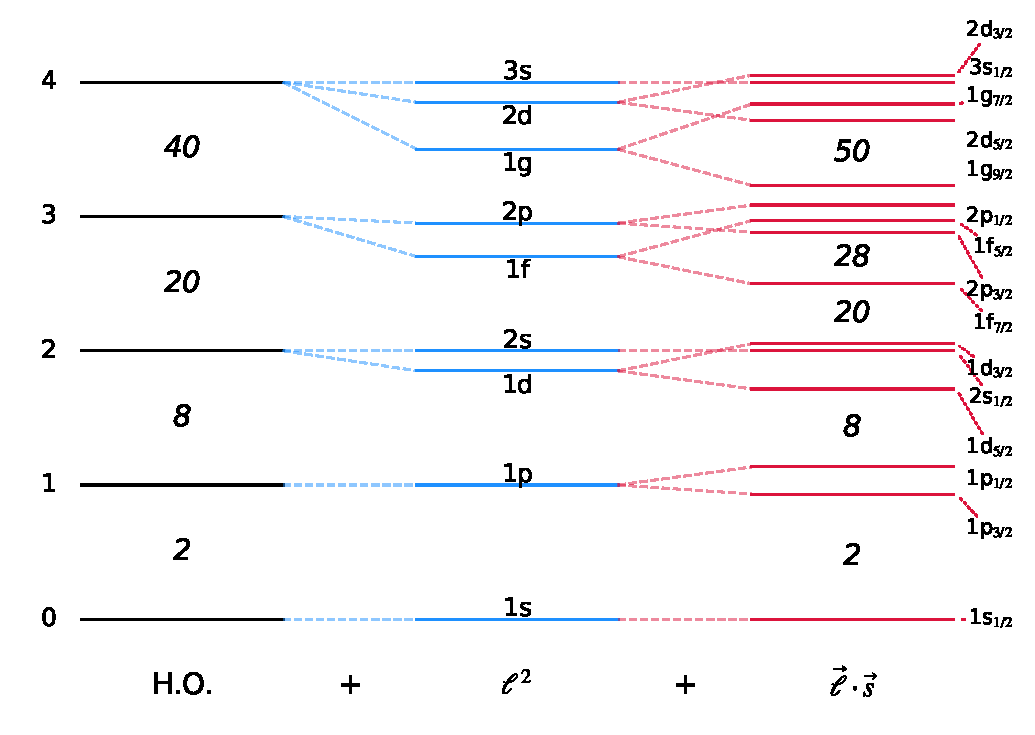
\includegraphics[width=3.33\linewidth]{Imagenes/Shell_model.pdf}};
    \end{tikzpicture}
    \captionof{figure}{modelo de capas de Goeppert-Mayyer \cite{GoepertMayer}, con la secuencia de números mágicos dibujada. }
    \label{fig:02-modelo_capas}
\end{minipage}
\vspace{0.9em}



\subsection{Núcleos ricos en neutrones y protones}

Los núcleos ricos en un tipo particular de nucleón (proton o neutrón) son sumamente intersantes, no solo porque son fundamentales a la hora de entender los procesos r astrofísicos \cite{THIELEMANN2011346} (proceso de captura rápida de neutrones) o los procesos rp (captura rápida de protones). Los procesos r son responsables  de la creación de la mayor parte de núcleos muy pesados $(60<A)$, que se dan en la expansión tras un colapso del núcleo de una supernova, o la descompresión de la materia neutrónica emitida por la fusión de una estrella binaria compacta de neutrones, mientras que los procesos rp ocurren hacia el final de las estrellas supermasivas, novas y en estrellas de neutrones, produciendo núcleos con A hasta $\sim$127. 

Además revelan nuevas estructuras nucleares (halos nucleares, modificación del orden de las capas nucleares y números mágicos...) que son muy interesantes desde el punto de vista teórico. 

Estas nuevas estructuras nucleares ponen a prueba modelos teóricos y arrojan información necesaria para adaptar modelos fenomenológicos que permitirán obtener resultados teóricos a otros núcleos ricos en neutrones imposibles de medir en experimentos actualmente por la incapacidad actual de producirlos (debido a su baja estabilidad y su falta de estados ligados). 

La mayor parte de estructuras exóticas la encontramos en la \textit{dripline}, tanto de protones, como de neutrones. Decimos que un núcleo ligado está en el límite de la \textit{dripline} de neutrones cuando añadir un neutrón más produce un estado no ligado, es decir, con energía de ligadura de neutrones negativa, exceptuando los casos en los que añadir dos neutrones produzca un estado ligado. De manera análoga para los protones. En la \cref{fig:02-dripline} podemos ver la dripline de protones y neutrones dibujada en la carta nuclear. 


Los núcleos cerca de la \textit{dripline} presentan formas exóticas, comportamientos anómalos que no son vistos en núcleos en la estabilidad. Entre estos comportamientos encontramos los núcleos halo. 

\begin{figure}[H]
    \centering
    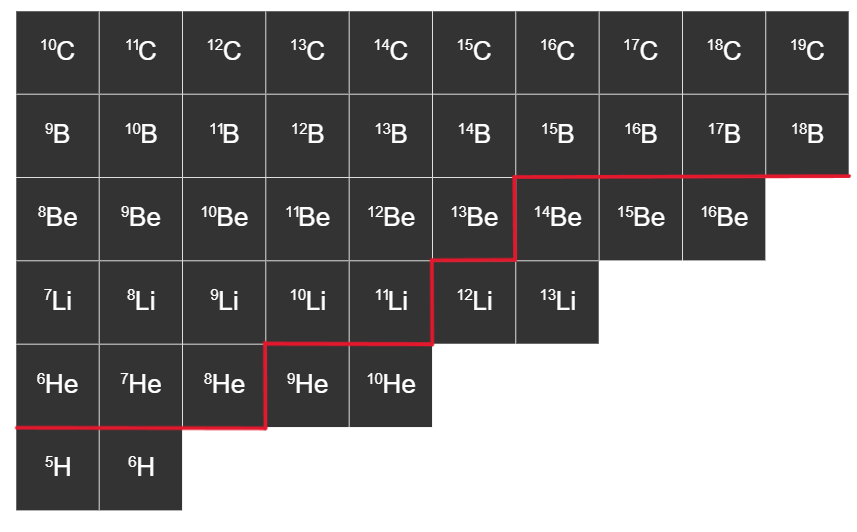
\includegraphics[width=0.5\linewidth]{Imagenes/NuclearChart.png}
    \caption{Dripline de neutrones (linea roja) para átomos ligeros, usando datos de \cite{Huang_2021} y la aplicación web \cite{nuclear_chart_colorful}.}
    \label{fig:02-dripline}
\end{figure}



Existen muchas maneras de obtener información acerca de la \textit{dripline}. Por un lado encontramos decaimientos beta, que nos permiten conocer la masa, espín y momentos angulares de dichos núcleos. Por otro lado las interacciones y secciones eficaces elásticas nos hablan acerca el radio y distribuciones de densidades, las distribuciones a diferentes energías y momentos angulares la presencia de núcleos halo. Las reacciones inelásticas de trasferencia o resonancias elásticas nos pueden arrojar información acerca de estados nucleares no ligados \cite{JONSON20041}. Nosotros nos centraremos en los núcleos con un alto número de neutrones, cerca de la \textit{dripline} de neutrones.

\subsection{Núcleo halo}


El halo de neutrones es, en esencia, una manifestación del efecto túnel cuántico, que surge cuando un estado nuclear ligado se encuentra muy próximo al continuo energético \cite{tanihata2023halo}.  Se entiende como una estructura formada por pocos cuerpos, un núcleo central (core) fuertemente ligado y uno o más nucleones externos débilmente ligados. A los núcleos formados por dos nucleones y un \textit{core}, tal que el estado con un núcleón y un \textit{core} es no ligado \cite{tanihata2023lowEnergyHalo} lo llamamos \textbf{núcleo Borremeano}, y podemos encontrar entre ellos $^6$He, $^{11}$Li, $^{14}$Be y $^{17}$B. 



Para que se de una estructura de halo se necesita una combinación de energía de ligadura de neutrones muy pequeña ($<1$ MeV) y una fuerza de corto alcance (como es la fuerza nuclear) \cite{tanihata2023halo}, que por ejemplo en el caso del $^{11}$Li es de $S_{2n}=369.15(65)$ keV \cite{PhysRevLett.101.202501}. Además, los núcleos halo deben estar en órbitas de bajo momento angular ($l =0,1$), es decir, ondas S y P. Esto es importante porque la barrera centrífuga de valores de $l$ alto inhibe la creación de núcleos halo \cite{tanihata2023halo}. El requerimiento de que la energía de ligadura sea pequeña hace que la mayor parte de los halos solo puedan tener uno o dos neutrones orbitando. Dicha combinación de factores permite que la función de onda del neutrón tenga una probabilidad significativa de encontrarse fuera del potencial nuclear, en regiones que serían prohibidas clásicamente alrededor del \textit{core} núcleo. Esto a su vez conduce a que el tamaño del núcleo sea más grande de lo normal, como se puede ver en la \cref{fig:02-radio_litio11}.

\begin{figure}[H]
    \centering
    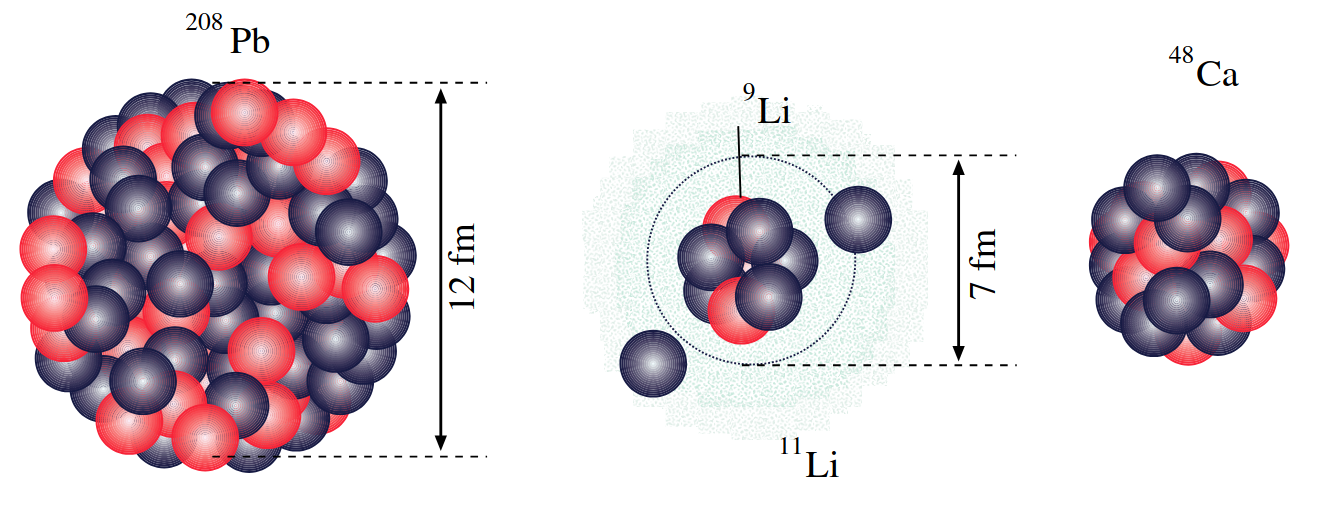
\includegraphics[width=0.9\linewidth]{Imagenes/Litio11.png}
    \caption{tamaño de diferentes núcleos, destacando el gran radio del litio 11 para su bajo número atómico.}
    \label{fig:02-radio_litio11}
\end{figure}

Precisamente esto fue demostrado en 1985 por Tanihata \textit{et al} \cite{Tanihata1985PLB} y \cite{Tanihata1985PRL}. Para el $^{11}$Li, que por aquel entonces era un candidato a ser un núcleo halo. En este experimento hallaron que su radio era un 30\% mayor que el núcleo $^{9}$Li. Teóricamente los núcleos en este estado manifiestan una interacción leve entre \textit{core} y halo \cite{JONSON20041}, y que por tanto la distribución de carga debía ser similar entre el \litioNueve \ y el \litioOnce . Esto fue probado por ISOLDE, en el CERN, estudiando el momento cuadrupolar eléctrico \cite{ARNOLD199216} y momento dipolar magnético \cite{Arnold:180144} a través de decaimientos beta. Se había predicho además que la presencia de halos estarían asociadas a grandes secciones eficaces, lo cual también fue demostrado experimentalmente. 


\subsection{Litio 10 y Litio 11}

El $^{10}$Li es un estado no ligado, lo que implica que solo puede vivir a través de estados resonantes en algún tipo de reacción. En principio el \litioOnce en su estado fundamental (\textit{ground state}), según el modelo de capas típico, debería tener una componente principal de $1p_{1/2}$ tal y como mostramos en \cref{Fig:2-Li10_1}. Sin embargo es sabido que debido al carácter tan exótico del \litioDiez  es de esperar un reordenamiento de las capas, por lo que es posible que el término con $2s_{1/2}$ de lugar a un estado con menos energía, como se ve en \cref{Fig:2-Li10_2}.

¿Por qué es interesante conocer el núcleo no ligado $^{10}$Li? Por que las función de ondas del $^{11}$Li puede expresarse en realidad como una superposición de diferentes resonancias del $^{10}$Li y un neutrón que ocupa una de las capas definiendo el espín-paridad del estado que observamos \cite{SANETULLAEV2016481}. Así pues, el estado fundamental del \litioOnce estará formado por el acoplo del estado del litio 10 y varios posibles estados orbitales del neutrón restante. El modelo de capas predice que las dos componentes que más contribuyen al estado fundamental son los orbitales $2s_{1/2}$ y $1p_{1/2}$, tal que

\begin{equation}
    \vert^{11}\text{Li}_{\text{g.s}}\rangle = \alpha\vert ^{10}\text{Li} \otimes \nu(2\text{s}_{1/2})\rangle\; + \beta\vert ^{10}\text{Li} \otimes \nu(1\text{p}_{1/2})\rangle\; + \cdots \label{Ec:02-Litio11}
\end{equation}
$\alpha$ y $\beta$ nos dan una medida de cuanto afectan estas componentes al estado fundamental. 

El reordenamiento producido por el uso de términos adicionales, como podrían ser las interacciones tensoriales y \textit{pairing} \cite{tanihata2023tensor} llevan a que el estado $2s_{1/2}$ se introduzca entre el $1p_{3/2}$  y el $1p_{1/2}$. Fuere cual fuere el término que origina el reordenamiento, lo que si sabemos es que el modelo de capas evoluciona a medida que nos movemos hacia la \textit{dripline}, lo que desplaza la energía de los orbitales y la posición de los números mágicos.

 %Based on this model the mixing of s- and p-waves are successfully explained as a Pauli blocking effect by the tensor interactions and pairing interactions. Under this model, as shown in Fig. 8, the ground state of 9 Li includes configurations denoted as “Pairing” and “Tensor” in addition to 0p-0 h configurations. “Pairing” configuration has a large two-neutron amplitude in 1p1/2 orbital. “Tensor” configuration has a proton and a neutron in 1p1/2 orbital excited from 1s1/2 orbital

\begin{minipage}{0.48\linewidth}
    \centering
    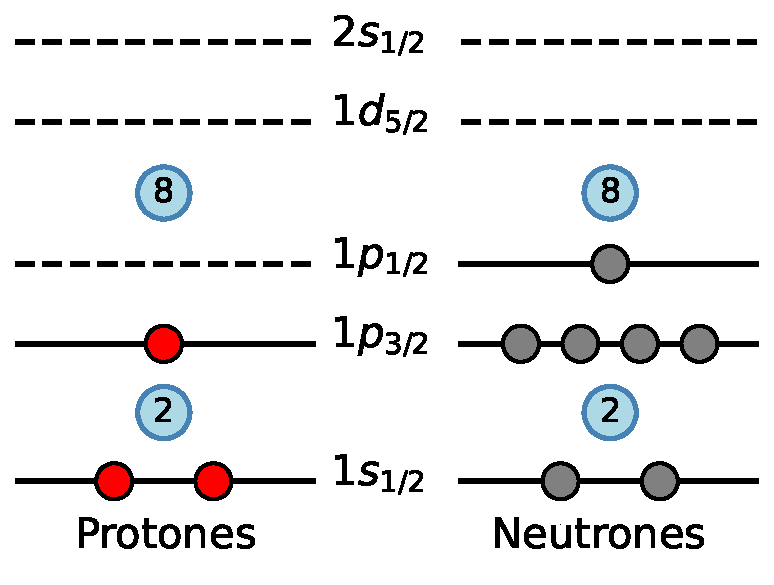
\includegraphics[width=1.0\linewidth]{Imagenes/Capas_10Li.pdf}
    \captionof{figure}{Capas del $^{11}$Li cuando le arrancamos un neutrón según el modelo de capas tradicional.}
    \label{Fig:2-Li10_1}
\end{minipage}
\hfill
\begin{minipage}{0.48\linewidth}
    \centering
    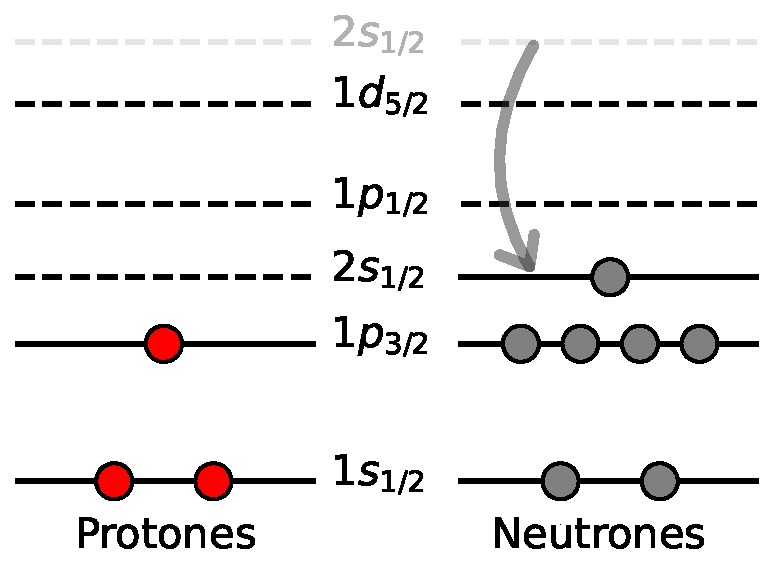
\includegraphics[width=1.0\linewidth]{Imagenes/Capas_10Li2.pdf}
    \captionof{figure}{Capas del $^{11}$Li cuando le arrancamos un neutrón según el modelo de capas modificado.}
    \label{Fig:2-Li10_2}
\end{minipage}
\vspace*{0.5cm}

Existen diferentes formas de explorar los estados resonantes, siempre a partir de reacciones de trasferencia, que son aquellas que suceden entre dos núcleos en su estado fundamental y que se trasfieren algún tipo de nucleón \cite{Tanihata2023DirectNuclearReactions}. Un ejemplo podría ser $^{9}\text{Be}(^{9}\text{Be},^{8}\text{B})^{10}\text{Li}$. Diferentes experimentos se pusieron en marcha para poder hallar cual era el estado fundamental y cuales los estados excitados del \litioDiez, si el $1p_{1/2}$ o el $2s_{1/2}$. Algunas de las reacciones probadas fueron $^{9}\text{Li}(\text{d},\text{p})\text{Li}$ o $^{10}\text{Be}^{12}(\text{C}, ^{12}\text{N})^{10} \text{Li}$. La mayor parte de estas mostró que efectivamente el primer estado excitado es el $1p_{1/2}$ mientras que el estado fundamental era el $2s_{1/2}$ \cite{SANETULLAEV2016481}. Las reacciones anteriores no son capaces de estudiar el grado de influencia tenían estas resonancias en el $^{11}$Li, por lo que había una necesidad de buscar reacciones que sí lo hicieran. 

%occur when a nucleon or a cluster of nucleons initially in a bound state of one of the two nuclei ends up in a bound state of the other nucleus

A través de reacciones que quiten neutrones al $^{11}$Li, tal y como pueden ser  $^{11}$Li(p,d)$^{10}$Li o $^{11}$Li(d,t)$^{10}$Li se podría estudiar esta interacción neutrón-\litioDiez, a través de la ocupación de los orbitales, que podemos obtener gracias a las secciones eficaces.

%eu non o entendín moi ben. se te atreves podes explicar moi brevemente que as reaccións de transferencia permiten acceder directamente á ocupación ou non ocupación dos orbitais mediante as seccións eficaces experimentais. -> A ver si lo hago



\subsection{Reacción de transferencia $^{11}$Li(d,t)$^{10}$Li}

La reacción en la que nos vamos centrar nosotros es

\begin{equation}
   {}^{11}\text{Li} + d \to t + {}^{10}\text{Li}
\end{equation}
particularmente interesante dentro del estudio del \litioOnce debido a su capacidad para proporcionar información directa sobre los espines y paridad del neutrón del \litioOnce a través de su eliminación. Además, a diferencia de muchas reacciones que sólo permiten estudiar el espectro excitado de \({}^{10}\text{Li}\), esta reacción accede directamente a las configuraciones de un solo neutrón en \({}^{11}\text{Li}\), lo que nos permite obtener el factor espectroscópico que nos permite hallar $\alpha$ y $\beta$ de \cref{Ec:02-Litio11}, o lo que es lo mismo, la probabilidad de que dicho neutrón esté en uno y otro orbital. 
 

¿Por qué es relevante estudiar \({}^{11}\text{Li}(d,t){}^{10}\text{Li}\)?
\begin{itemize}
    \item Permite investigar el papel de los estados resonantes de \(^{10}\text{Li}\) en la estructura del halo de \(^{11}\text{Li}\). Dado que $^{10}\text{Li}$ es inestable y no tiene un estado ligado, su estudio experimental es muy complicado, y esta reacción permite observar sus resonancias de forma más directa. \cite{SANETULLAEV2016481}.
    
    \item La eliminación de un neutrón del \(^{11}\text{Li}\), trasfiriéndolo al \(^{10}\text{Li}\), nos permite obtener características específicas de momento angular y energía, mostrando la naturaleza de las configuraciones \(s_{1/2}\) y \(p_{1/2}\) en el estado fundamental de \({}^{11}\text{Li}\), i.e. nos permite conocer la función de ondas en el estado fundamental.  \cite{CASAL2017307}. 
    
    \item Es sensible a los factores espectroscópicos, es decir, permite medir el grado de ocupación una cierta configuración de un neutrón y \({}^{10}\text{Li}\) en el estado fundamental de \({}^{11}\text{Li}\), lo cual no es accesible en muchas otras reacciones. \cite{SANETULLAEV2016481}. De conocer todos los factores espectroscópicos podríamos conocer  podríamos obtener la probabilidad de ocupación de uno u otro orbital.
\end{itemize}
Además, al igual que las otras funciones de trasferencia, permite ajustar mejor los parámetros de los modelos fenomenológicos, guiando los modelos existentes y las interacciones nucleares, con el objetivo de caracterizar correctamente otros núcleos exóticos cerca de la \textit{dripline} de neutrones.

%En resumen, la reacción \({}^{11}\text{Li}(d,t){}^{10}\text{Li}\) no sólo aporta datos sobre los estados de \({}^{10}\text{Li}\), sino que se convierte en una herramienta crucial para entender cómo se configura el halo en \({}^{11}\text{Li}\), permitiendo extraer porcentajes de contribuciones tipo \(s_{1/2}\) y \(p_{1/2}\), y estudiar la ruptura del cierre de capa en \(N=8\). Por ello, tiene una relevancia singular dentro de la física nuclear de sistemas exóticos, tanto para 

